% comment out (using a %) exactly 1 of the 2 lines immediately below
%\documentclass[handout]{beamer}   % to produce a handout
\documentclass{beamer}             % to produce slide show with pauses etc.

%\usepackage{xeCJK}
%\setCJKmainfont{SimSun}

\usepackage{ucltemplate}
\usepackage{hyperref}  % to enable hyperlinks to websites to be produced.

\setbeamertemplate{footline}{\normalsize\hfill\insertframenumber/\inserttotalframenumber} % add slide number

\setbeamertemplate{navigation symbols}{} %no navigation symbols on the bottom right of the slides

% To force beamer to include table and figure numbers
% This is just for the purposes of the STAT0034 workshop: usually one would not want cross-references in a presentation
\setbeamertemplate{caption}[numbered]

% for nice-looking inequality signs
\let\leq=\leqslant
\let\geq=\geqslant

% Choose the color you like
\usecolortheme{lightblue}
%\usecolortheme{black}
%\usecolortheme{darkred}

% Pick a colour (a blue) for the weblinks
\definecolor{links}{HTML}{2B65EC}
\hypersetup{colorlinks, linkcolor=, urlcolor = links}

% Information for title page
\title{\bf \Large An introduction to \LaTeX}
\author[]{Ricardo Silva}
%\institute{Department of Statistical Science}
\date{STAT0034, January 2020}

% Start the document
\begin{document}

% Every slide is defined within a frame environment which
% start with \begin{frame} and ends with \end{frame}
\begin{frame}
\titlepage

\begin{quote}
 ``\ldots intended for the creation of beautiful books -- and especially for books that  contain a lot of mathematics'' 
\end{quote}
\begin{center}Donald E. Knuth on \TeX \,(the original version of \LaTeX). \end{center}

\end{frame}

\begin{frame}{\LaTeX}

% Every list of remark can be defined within an itemize environment which
% start with \begin{itemize} and ends with \end{itemize}
\begin{itemize}
\setlength{\itemsep}{.3cm}
\item LaTeX (pronounced lay-tek) is a document preparation system for TeX
\item Tex is a typesetting system designed by Donald Knuth and released in 1978
\item LaTeX refers only to the language, not to the editor used to write LaTeX documents
\item LaTeX documents are plain text files with the extension .tex
\item Web site: {\tt www.latex-project.org}
\item LaTeX is free and widely used in academia
\end{itemize}
\end{frame}


\begin{frame}{Why use \LaTeX \,instead of MS Word?}

% A picture can be included as an pdf using \includegraphics
% The construction below with tabular and minipage is one
% way to create a good layout.
\begin{tabular}{cc}
\begin{minipage}{1.5in}
{According to some ...}
\end{minipage}
&
\begin{minipage}{3in}
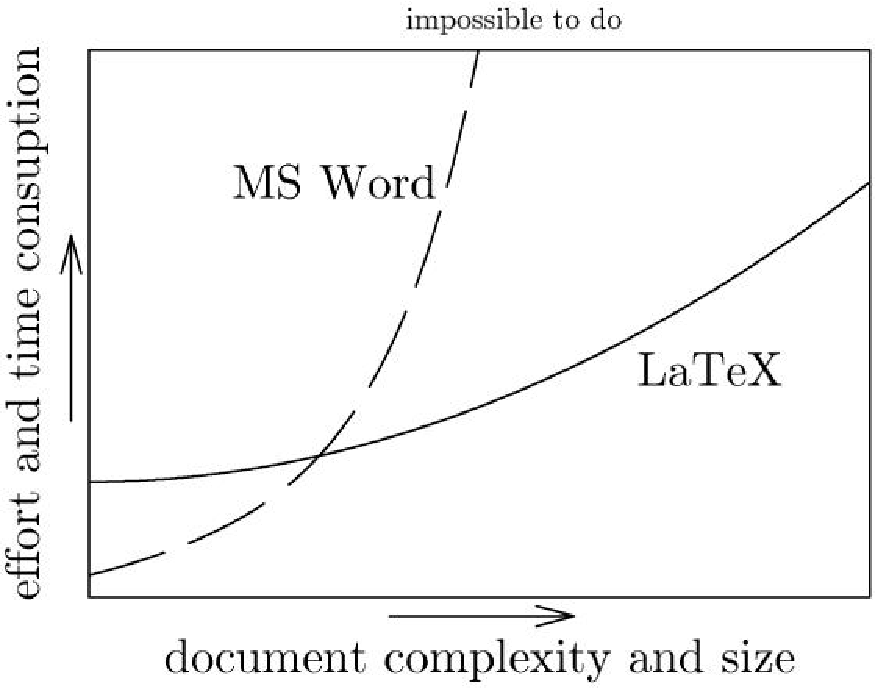
\includegraphics[width=2.75in]{latex_vs_word.pdf}
\end{minipage}
\end{tabular}
\end{frame}


\begin{frame}
\begin{itemize}
\setlength{\itemsep}{.2cm}
\item LaTeX produces good-looking mathematics %\pause
\item LaTeX produces nice-looking documents %\pause
\item It can easily be set up to update automatically references to sections, tables, figures %\pause
\item BibTeX: automatic handling of references to papers/books %\pause
\item {\bf \alert{Main philosophy:}} content is separate from layout. Write content without worrying (much) about appearance.
  One can change the appearance of the whole document easily \\
\medskip
\alert{\bf ... and ...}
\medskip
\item Using LaTeX pleases LaTeX-users. In some fields LaTeX is the norm
\end{itemize}
\end{frame}


\begin{frame}
\ldots \alert{\bf but}\\
\medskip
\begin{itemize}
\setlength{\itemsep}{.3cm}
\item MS Word editor for formulas has improved in recent years
\item MS Word: you see what your document looks like as you edit it
\item Some journals/companies do not accept/use LaTeX
\item For LaTeX you need to do a couple of steps to see the final document:
\begin{itemize}
\setlength{\itemsep}{.2cm}
\item Either \ \ \alert{\bf .tex $\rightarrow$ .pdf}
\item or\ \  \alert{\bf .tex $\rightarrow$ .dvi $\rightarrow$ .pdf or .ps}
\item Then view \alert{\bf .pdf or .ps file}
\end{itemize}
\end{itemize}
\end{frame}


\begin{frame}{\LaTeX \ use in journals}
\begin{itemize}
\setlength{\itemsep}{.25cm}
\item Nature:
\begin{quote}
Our preferred format for text is Microsoft Word... If you have prepared your paper using TeX, please convert to PDF format and upload the PDF
\end{quote}
\item Journal of the American Statistical Association:
\begin{quote}
Manuscripts submitted in LaTeX should use the ``article'' style and should not use any special macros. Authors should use BiBTeX to prepare references whenever possible. Please use {natbib.sty}, and either {plain.bst} or {apalike.bst} ...
\end{quote}
\item Journal of the Royal Statistical Society Series C:
\begin{quote}
A complete LaTeX style file ... is available to download .. but it is not compulsory to use it
\end{quote}
\end{itemize}
\end{frame}


\begin{frame}{Getting \LaTeX}
\begin{itemize}
\setlength{\itemsep}{.5cm}
\item You need to download MikTeX from \url{www.miktex.org}
\item Choose your programme/editor
\begin{itemize}
 \item Free TeXstudio from \url{http://texstudio.sourceforge.net}
 \item Free TeXworks from \url{http://www.tug.org/texworks/} 
 \setlength{\itemsep}{.25cm}
 \item Free TeXMaker from \url{https://www.xm1math.net/texmaker/}
 \item Almost free WinEdit from \url{www.winedt.com}
 \item RStudio! and etc. ....
\end{itemize}
\item These programmes include easy click-able routines for building pdf from a .tex file
%\item {\bf Alternative}: get installation disk from departmental Systems Administrator Chakkapas Visavakul
\end{itemize}
\end{frame}

\begin{frame}{Share the \LaTeX \ knowledge}
\begin{itemize}
\setlength{\itemsep}{.5cm}
\item Do not write a LaTeX file from scratch! Use an existing document/template and adapt
\item \alert{\bf Annotated .tex file for these slides on Moodle}
\item \alert{\bf Annotated .tex file for an MSc report also on Moodle}
\item Use tips from other people or search the web when you encounter a problem
\end{itemize}
\end{frame}

\begin{frame}
Next some explanation and tips for writing LaTeX...
\end{frame}


\begin{frame}[containsverbatim]{Maths in the main text}
\begin{itemize}
\setlength{\itemsep}{.5cm}
\item Distinguish math symbols in main text. Dollar signs denote math mode: \verb!$x$! gives $x$ (rather than x)
\item Greek symbols: \verb!$\alpha$! gives $\alpha$, \verb!$\Omega$! gives $\Omega$ etc.
\item Mathematical operators:
\begin{itemize}
\setlength{\itemsep}{.25cm}
\item \verb!$1/x$! gives $1/x$
\item \verb!$x^\alpha$! gives $x^\alpha$
\item \verb!$x^{-1}$! gives $x^{-1}$
\item \verb!$\log x$! gives $\log x$
\item \verb!$\frac{x}{y}$! gives $\frac{x}{y}$
\item \verb!$\displaystyle\frac{x}{y}$! gives $\displaystyle\frac{x}{y}$
\end{itemize}
\end{itemize}
\end{frame}

\newcommand{\e}{ {\rm e} } % a useful way to produce your own LaTeX commands
\begin{frame}[containsverbatim]
\begin{itemize}
\setlength{\itemsep}{.25cm}
\item You can define your own symbols/commands:\\
\begin{center}
\verb!\newcommand{\e}{ {\rm e} }!
\end{center}
Compare
\begin{center}
\verb! f_X(x) = \lambda \e^{-\lambda x}, \quad x > 0. !
\end{center}
\medskip
\[ f_X(x) = \lambda \e^{-\lambda x}, \quad x > 0.  \]
with
\begin{center}
\verb! f_X(x) = \lambda e^{-\lambda x}, \quad x > 0. !
\end{center}
\medskip
\[ f_X(x) = \lambda e^{-\lambda x}, \quad x > 0.  \]
\end{itemize}

\end{frame}

\begin{frame}[containsverbatim]{Maths in displayed equations}

\begin{verbatim}
\begin{equation}
  f_X(x) = \lambda \, \e^{-\lambda x}, \quad x > 0.
  \label{eqn:one} % label for equation
\end{equation}
This comment refers to equation (\ref{eqn:one}).
\end{verbatim}

\vspace{.5cm}
\hrule
\vspace{.5cm}

\begin{equation}
  f_X(x) = \lambda \, \e^{-\lambda x}, \quad x > 0.
  \label{eqn:one} % label for equation
\end{equation}
This comment refers to equation (\ref{eqn:one}).

\end{frame}



\begin{frame}[containsverbatim]{Multi-line displayed equations}

\begin{verbatim}
\begin{eqnarray}
L(\lambda)
&=&\prod_{i=1}^n\lambda\e^{-\lambda x_i}\nonumber\\
&=&\lambda^n \exp\left\{-\lambda \sum_{i=1}^n x_i\right\}.
\label{eqn:two}
\end{eqnarray}
\end{verbatim}

\vspace{.1cm}
\hrule
\vspace{.1cm}
\begin{eqnarray}
 L(\lambda) &=& \prod_{i=1}^n \lambda \e^{-\lambda x_i} \nonumber \\ % use \nonumber for no equation number
 &=& \lambda^n \exp \left\{-\lambda \sum_{i=1}^n x_i \right\}. \label{eqn:two}% \left\{ ... \right\} sizes brackets
\end{eqnarray}

\end{frame}

\begin{frame}[containsverbatim]
\begin{verbatim}
\begin{eqnarray*}    % eqnarray* for no equation numbers
P(M_n\leq z)
&=&P(X_1\leq z,X_2\leq z,\ldots,X_n\leq z)\\
&=&P(X_1 \leq z) \times \cdots \times P(X_n \leq z)\\
&=&{F(z)}^n.
\end{eqnarray*}
\end{verbatim}
\vspace{.1cm}
\hrule
\begin{eqnarray*}                         % eqnarray* produces no equation numbers
P(M_n \leq z)&=&P(X_1 \leq z,X_2 \leq z,...,X_n \leq z)  \\
    &=&P(X_1 \leq z)  \times \cdots \times P(X_n \leq z) \\
    &=&{F(z)}^n.
\end{eqnarray*}
\vspace{.05cm}
\hrule
\vspace{.15cm}
{Note: Mathematics should read just like sentences of text, with punctuation, i.e. commas, full stops etc.}
\end{frame}

\begin{frame}[containsverbatim]{Including a pdf file as a figure}

\begin{verbatim}
\begin{figure}[h]
  \centering
  \includegraphics[width=7.5cm, angle=0]{file1.pdf}
  \includegraphics[width=7.5cm, angle=0]{file2.pdf}
  \caption{Put helpful caption in here ...}
  \label{fig:name}
\end{figure}

Figure \ref{fig:name} shows ...
\end{verbatim}

\end{frame}


\begin{frame}[containsverbatim]{Example of a table in LaTeX}


%{\it Example of a table in LaTeX...}
\medskip
\begin{table}[h]
\centering
\begin{tabular}{lrcrl}\hline
model & neg. log-lik & d.f. & ALRS  & $p$-value \\ \hline
constant & 22763.20     &    &       &           \\
linear   & 22742.59     & 2  & 34.23 & 0.0037    \\
quadratic  & 22737.09     & 3  & 20.50 & 0.013     \\
cubic & 22737.02     & 4  & 2.09  & 0.72      \\ \hline
\end{tabular}
\label{tab:simple}
\caption{Summary of point process modelling in which the location parameter $\mu$ is modelled as a Legendre polynomial function of
longitude and latitude and $\sigma$ and $\xi$ are constant. The tests compare the model with the model in the row above.
Notation: neg. log-lik, negated maximised log-likelihood; d.f., degrees of freedom of the null chi-squared distribution; ALRS, adjusted likelihood ratio statistic.}
\end{table}
\end{frame}

\begin{frame}[containsverbatim]{A table}

\begin{verbatim}
\begin{table}[h]
\centering
\begin{tabular}{lrcrl}\hline
model & neg. log-lik & df & ALRS  & $p$-value \\ \hline
constant & 22763.20     &    &       &           \\
linear   & 22742.59     & 2  & 34.23 & 0.0037    \\
quadratic  & 22737.09     & 3  & 20.50 & 0.013     \\
cubic & 22737.02     & 4  & 2.09  & 0.72      \\ \hline
\end{tabular}
\label{tab:simple}
\caption{Summary of point process modelling in which ...}
\end{table}

Table \ref{tab:simple} shows ...
\end{verbatim}

\end{frame}


\begin{frame}[containsverbatim]{Miscellaneous stuff}
\begin{itemize}
\setlength{\itemsep}{.3cm}
\item Sections, graphs, tables, equations labelled using \verb!\label{name}! and cited using \verb!\ref{name}!
\item Nested files? (to avoid having one big LaTeX file):
\begin{verbatim}
\begin{document}
\input{section1.tex}
\input{section2.tex}
etc.
\end{document}
\end{verbatim}
\item \verb!\clearpage!  forces LaTeX to put in all figures/tables before starting on new text.  This can help to keep figures/tables close to where they are cited in the text
\item \verb!\hat{\theta}! gives $\hat{\theta}$
\item \verb!Y \sim N(0,\sigma^2)! gives $Y \sim N(0,\sigma^2)$
\end{itemize}
\end{frame}

\begin{frame}{References}
\begin{itemize}
\setlength{\itemsep}{.3cm}
  \item LaTeX has BibTeX, an automatic way to produce citations in the text, using a consistent format, and a list of references
  \item Put details of books/papers etc. in a bibliography .bib file
  \item Often you can download the BibTeX entry from the web
  \begin{itemize}
    \item from the publisher of an article or book
    \item using reference managing software, such as Mendeley \url{https://www.mendeley.com/}
  \end{itemize}
   \item Setup BibTeX when you first start writing
   \item Add citations as you go along: don't leave this until the end of your project
\end{itemize}
\end{frame}



\begin{frame}[containsverbatim]{Giving a talk using beamer}
\setbeamercovered{transparent}
\begin{itemize}
\setlength{\itemsep}{.5cm}
\item These slides have been produced using the LaTeX package \alert{\bf Beamer}
%\item The header has been adapted to incorporate UCL corporate logo.
%\item Beamer can produce Powerpoint-like effects
\item For a user's guide: Google search for {\it Beamer User Guide for version 3.57}
\item There is a lot on Beamer on-line. A nice example can be found at
\url{www.math.utah.edu/~smith/Beamer}
\item An alternative for making slides is using
\begin{verbatim}
\documentclass[landscape]{slides}
\begin{slide}
...
\end{slide}
\end{verbatim}
\end{itemize}
\end{frame}

\begin{frame}{Getting help}
\begin{itemize}
\setlength{\itemsep}{.5cm}
\item There are many websites devoted to LaTeX
\url{www.ctan.org/starter.html} is a good place to start
\item Specifically for maths see also
\url{www.math.uiuc.edu/~hildebr/tex/displays.html}

\item There are also books:

\begin{itemize}
\begin{footnotesize}
\setlength{\itemsep}{.25cm}
\item Kopka and Daly (2003)  {\it A Guide to LATEX: Tools and Technologies for Computer Typesetting}, Addison-Wesley
\item Lamport (1994)  {\it LATEX: a Document Preparation System : User's Guide and Reference Manual}, Addison-Wesley
\item Mittelbach, Goossens, Braams, and Carlisle  (2004) {\it The Latex Companion}, Addison-Wesley
\end{footnotesize}
\end{itemize}
\end{itemize}

\end{frame}


\begin{frame}
\begin{itemize}
\item There are R packages, e.g.\\
\setlength{\itemsep}{.5cm}
\begin{itemize}
\setlength{\itemsep}{.25cm}
\item Hmisc (\url{cran.r-project.org/web/packages/Hmisc}), and
\item xtable (\url{cran.r-project.org/web/packages/xtable}),\\
\end{itemize}
that have functions for converting numerical results into LaTeX code for tables
\item Automated on-line LaTeX table generator at \url{www.tablesgenerator.com}
\item The R package mathpix (\url{https://cran.r-project.org/web/packages/mathpix/index.html}) can convert typed or handwritten maths to LaTeX code
\end{itemize}
\end{frame}



\begin{frame}{Online \LaTeX}
\begin{itemize}
\setlength{\itemsep}{.5cm}
\item \alert{\bf Overleaf} is online system at \url{www.overleaf.com}
\item Can be linked to GitHub (\url{www.github.com}) to facilitate synchronisation with a local machine
\item OK for getting started, but long term: \alert{use your own editor, store your own files}
\begin{itemize}
\setlength{\itemsep}{.35cm}
\item[--] To be independent of on-line access and problems at \url{www.overleaf.com}
\item[--] To limit access to your {\it work in progress}
\end{itemize}
\end{itemize}
\end{frame}

\begin{frame}{Markdown and Jupyter Notebooks}
\begin{itemize}
\setlength{\itemsep}{.5cm}
\item \alert{\bf Markdown} is a simplified version of \LaTeX
\item For instance, to create an itemised list, just start sentences with an asterisk
\item Markdown is also used by {\bf Jupyter notebooks}, a way of integrating code and \LaTeX-like comments
      (``Jupyter'' stands for Julia/Python/R, the initial three languages targeted).  
      It's a very good way to keep track of your code as you progress in your MSc project.
      See a few examples of it in some of your STAT0030 labs.
\item A Markdown cheatsheet: \url{https://stationinthemetro.com/apps-and-scripts/markdown-cheat-sheet}
\item Project Jupyter webpage: \url{https://jupyter.org}
\end{itemize}
\end{frame}


\begin{frame}[containsverbatim]{Last-minute tips}
\begin{itemize}
\setlength{\itemsep}{.35cm}
\item Don't forget spell-checking! Different editors offer different options. Old schoolers can use {\tt aspell} for a plain tool
\item Don't use spacing in names of files or directories
\item Put your graph files where ``LaTeX can find them''. Either
\begin{itemize}
\item same directory as the main .tex file
\verb! \includegraphics[width=7cm, angle=0]{file1.pdf}! 
\item in a PLOTS directory
\verb! \includegraphics[width=7cm, angle=0]{PLOTS/file1.pdf}! 
\end{itemize}
\item Figures can be of extension .pdf and .eps. Depends on how you compile the .tex file. If you go directly from .tex to .pdf, then \alert{use .pdf figures}
\end{itemize}
\medskip
\end{frame}

\begin{frame}{Finally}
\begin{itemize}
\setlength{\itemsep}{.25cm}
\item I encourage you to use LaTeX for your project report
\item The initial startup time/effort is worth it in the longer term
\end{itemize}
\medskip
\begin{center}
\alert{\bf All the material from this workshop + template for an MSc project report are on Moodle}
\end{center}
\end{frame}

\end{document}



